
\section{Methodology}

In this study, a baseline algorithm is presented for comparative purposes. Subsequently, two valid alternative approaches are thoroughly examined. The first approach involves employing a customized Genetic Algorithm for hyperparameter tuning of a LSTM model, while the second approach utilizes Genetic Programming to directly infer potential relationships among variables from the data.

\subsection{Baseline}

The most basic model involves predicting the temperature for the next hour using a simple approach: returning the last observed temperature. This straightforward model is encapsulated by the equation:

\begin{equation}
    f(x_t, x_{t-1}, \ldots, x_{t-p+1}) = x_t
\end{equation}

\subsection{LSTM tuning using Genetic Algorithms}

The intricate relationships concealed within time series data pose a challenge for conventional neural networks, which often find it difficult to effectively model such sequences. In response to this challenge, Recurrent Neural Networks(RNN) emerge as a valuable solution, enabling the processing of sequential data and the integration of learned parameters from preceding time steps. Numerous studies have demonstrated the limitations of standard neural networks in handling weather-related time series data\cite{weather-lstm}, emphasizing the superior performance of more advanced RNN-based models, such as Long Short-Term Memory(LSTM) networks.

\begin{figure}[h]   
    \centering
    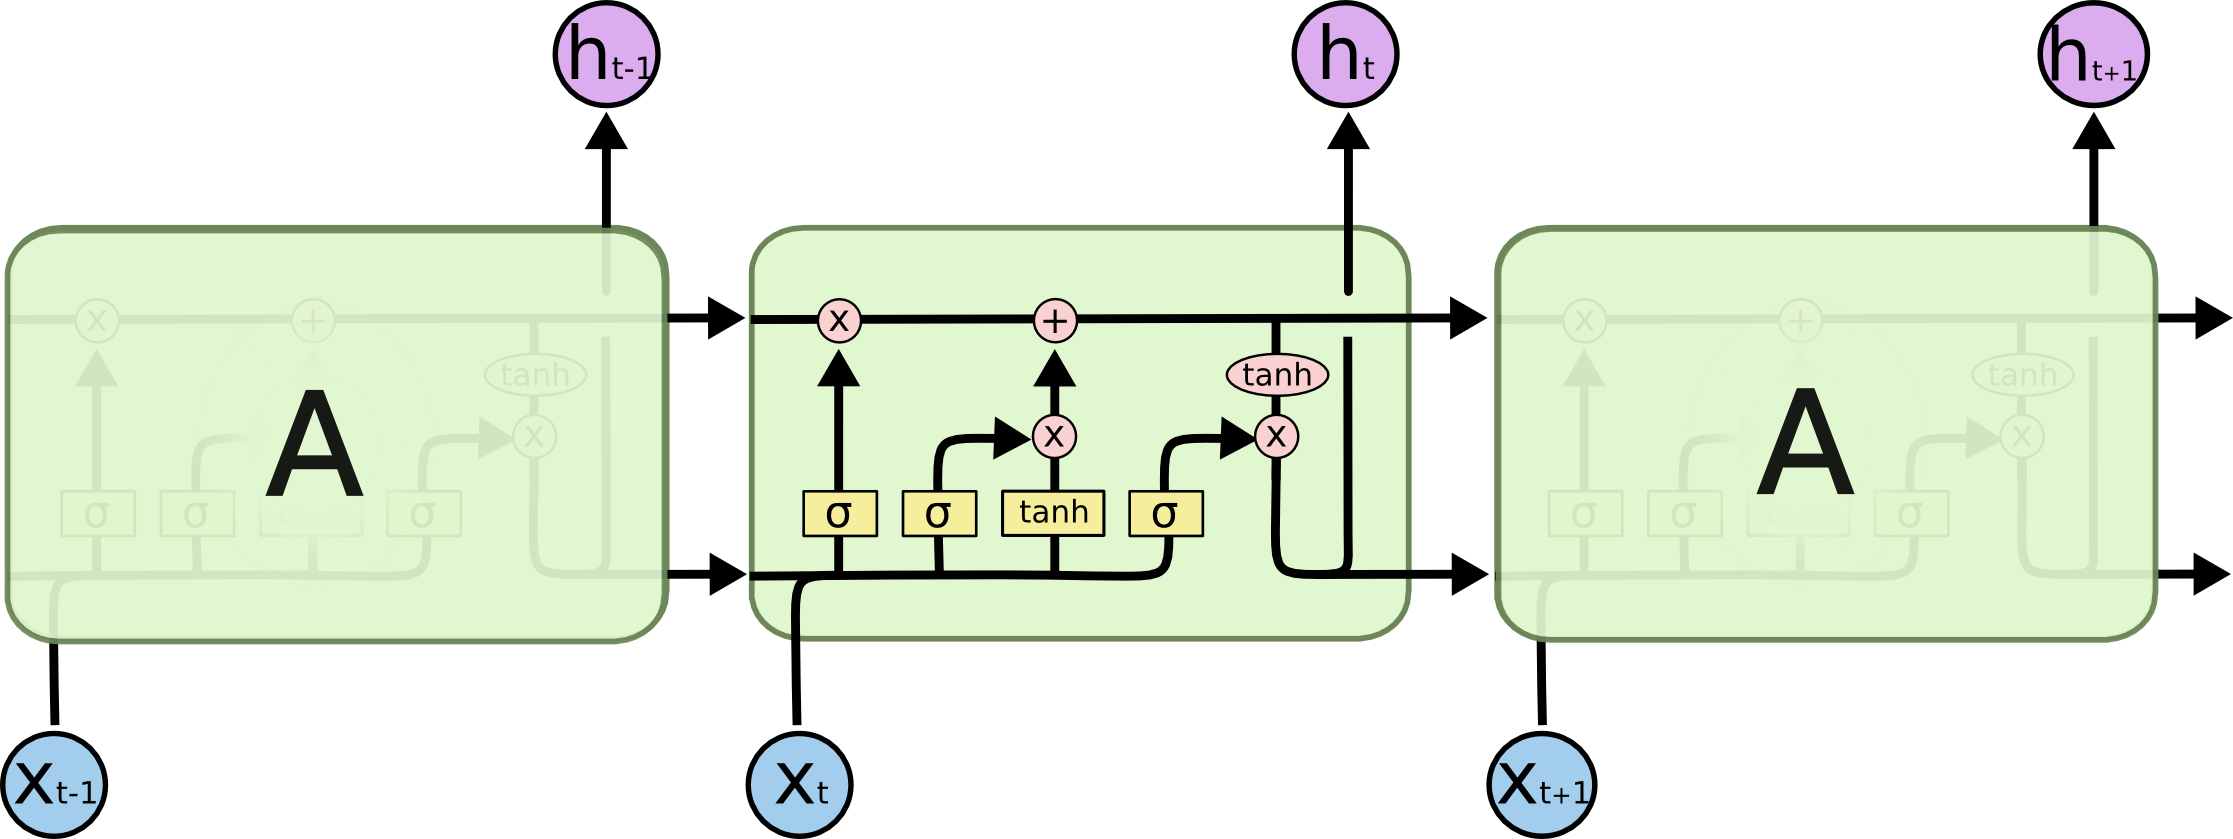
\includegraphics[width=0.4\textwidth]{LSTM-chain.png}
    \caption{The architecture of a LSTM.}
    \label{fig:lstm}
\end{figure}

Without entering into specific details, LSTM networks are explicitly crafted to capture and model long-term dependencies within sequences of information. The network incorporates loops, enabling the propagation and retention of information over time, essentially serving as a form of memory. In this specific context, a sequence refers to a subset of a weather time series with a length of $p$, denoted as $\{x_1, x_2, \ldots, x_p\}$, where $p < N$ represents the sequence length corresponding to the number of preceding weather samples used for prediction. At the end of the LSTM network, there is a linear layer that compresses the output into a single floating-point value, representing the ultimate temperature forecast. The entire architecture is trained via backpropagation, and the hyperparameters are detailed as follows:
\begin{itemize}
    \item \textbf{Sequence length}: the length of the sequence corresponding to the number of prior weather samples used for prediction.
    \item \textbf{LSTM hidden size}: the number of hidden units or neurons in each LSTM layer, determining the capacity of the model to capture complex patterns.
    \item \textbf{LSTM number of layers}: the number of stacked LSTM layers.
    \item \textbf{Optimizer learning rate}: the step size at which the optimizer adjusts the model weights during training.
    \item \textbf{Extra parameters list}: additional parameters beyond the outdoor temperature included as inputs, providing supplementary information for the model. Each element in the input sequence fed to the LSTM can be a vector of multiple features. Therefore, this hyperparameter aims to identify the weather parameters that enable the model to achieve optimal accuracy.
\end{itemize}

To employ genetic algorithms, various aspects must be defined, including the representation of the genotype for each individual, the selection mechanisms and the methods for individual mutation and crossover.


\subsubsection{Encoding of the Genotype}
In this specific context of hyperparameter tuning, the genotype is represented as an array containing the aforementioned hyperparameters, maintaining the same order. The order within the array is significant, as both the mutation and crossover operators are specifically tailored for this specific order.

\subsubsection{Crossover}
Crossover plays a pivotal role in emphasizing exploitation by combining optimal parts from different individuals. In this context, a uniform crossover operator is employed, selecting elements from the first and second individuals with equal probability.\\
% \subsubsection{Crossover}
% This method combines an arithmetic crossover operator for the initial four parameters and a uniform crossover operator for the last parameter. The arithmetic crossover computes the mean value of the two individuals for the first four parameters, while the uniform crossover randomly selects elements from the first and second individuals with equal probability for the last parameter.\\


\subsubsection{Mutation}
The first three parameters of the genotype (sequence length, LSTM hidden size, and LSTM number of layers) are integers, while the remaining ones are a float (the learning rate) and an array (the set of extra parameters). Considering the distinct nature of each gene in the genotype, a custom mutation operator has been implemented. It introduces an integer/float perturbation following a normal distribution to the integer/float genes, respectively, with a magnitude proportional to a predefined standard deviation provided by the user. For the last element in the genotype, the set of extra parameters, one element is probabilistically removed and added based on a certain probability.\\


\subsubsection{Selection} 
In the context of parent selection, tournament selection has been employed, wherein individuals are randomly sampled and compared against each other in tournaments of size $K$. The fittest individual from each tournament is then chosen as a parent for the genetic operations. Moreover, survivor selection follows an elitism strategy, aiming to preserve the best individuals from the previous generation. \\


\subsubsection{Algorithm} 
The genetic algorithm can be outlined as follows:

\begin{enumerate}
    \item Randomly sample an initial population of individuals.
    \item Evaluate the fitness of all individuals in the population.
    \item Select parents for reproduction through tournament selection(parent selection).
    \item With a probability $p_{c}$, choose two individuals from the parents' pool and return a single individual by applying the crossover operator. The new individual is then reintroduced into the parent pool.
    \item With a probability $p_{m}$, pick one individual from the parents' pool and subject it to mutation.
    \item Select individuals for the next generation by employing elitism as the survivor selection method.
    \item Repeat from step 2 until a termination condition is met, such as reaching a specified number of generations.
\end{enumerate}


\subsection{Genetic Programming}
The prior approach, which uses deep learning to address the time series weather temperature forecasting problem, lacks a crucial aspect: interpretability. This lack push the exploration of a second methodology centered on Genetic Programming, with the primary goal of establishing an interpretable model for the problem at hand.

In Genetic Programming, individuals are characterized by tree-based structures that represent a program or equation. The objective is to evolve a computer program or equation capable of solving the problem by directly deducing relationships within the data, without any prior assumptions about the model. However, a significant challenge encountered in Genetic Programming lies in the requirement for a large population of individuals. The dimensions of the evolved programs or equations can quickly increase, necessitating a substantial number of individuals within the population to adequately navigate and explore the search space.

In this study, the objective of Genetic Programming is to evolve an arithmetic expression that effectively models the intricate relationships among various weather parameters. This evolved tree-based structure representing an expression should have the capacity to predict the outdoor temperature for the subsequent hour, relying solely on prior observations.


The tree-based structure consist of nodes, where:
\begin{itemize}
    \item The leaves of the tree derive values from the \textbf{terminal set} $T$, encompassing constants and all variables relevant to the problem. In the problem examined in this study, the terminal set is defined as $\{x_t, x_{t-1}, \ldots, x_{t-p+1}, e\}$, where $p$ represents the number of preceding samples used for prediction, and $e$ is an ephemeral constant randomly initialized.
    \item The inner nodes represent functions that establish relationships among nodes in the terminal set. Each function has an arity, indicating the number of arguments it accepts. In this instance, the \textbf{function set} is denoted as $F$ and contains the four basic arithmetic operations and the trigonometric functions, $\sin$ and $\cos$. Due to the impracticality of a priori checking all potential inputs with Genetic Programming, the division operator has been redefined to prevent a zero division error.
\end{itemize}

Since the genotype is represented as a tree-based structure, standard mutation and crossover operations need to be tailored accordingly. In the case a one-point crossover is used, wherein a random crossover point is chosen in each individual, and the sub-trees rooted at the selected point are exchanged between the individuals. Regarding mutations, a customized mutation operator is employed, incorporating three mutation strategies randomly chosen with equal probability:

\begin{itemize}
    \item \textbf{Shrink}: a random node in the tree is selected, and the entire sub-tree is replaced with a single node.
    \item \textbf{Increase}: this strategy inserts a new branch at a random position in the mutated individual.
    \item \textbf{Ephemeral Mutation}: this mutation alters one of the ephemeral variables by applying a random mutation.
\end{itemize}

The rationale behind this mutation operator is to mitigate the bloat problem. This approach gives trees the flexibility to grow or shrink with an equal probability, thus preventing excessive growth.


